\section{Scan and Fold}
\begin{algorithm}
    \caption{Scan operator for a binary function $f: \mathcal{T}_2 \times \mathcal{T}_1 \to \mathcal{T}_2$. The notation of using a backslash is borrowed from \citet{iverson62,iverson79}. Note that we prepend the initial value to the returned sequence. If $\mathcal{T}_1 = \mathcal{T}_2$, we take the first value of $x$ as the initial value.}
    \label{alg:scan}
    \begin{algorithmic}[1] \Function{$[f: \mathcal{T}_2 \times \mathcal{T}_1 \to \mathcal{T}_2]\backslash$}{$t_0: \mathcal{T}_2$, $x: \mathcal{T}_1^N$} $\to \mathcal{T}_2^{N+1}$
            \State $y: \mathcal{T}_2^{N+1}$
            \State $y_1 \gets t_0$
            \Statex
            \State $t: \mathcal{T}_2 \gets t_0$
            \For{$i \gets 1,N$}
                \State $t \gets f(t, x_i)$
                \State $y_{i+1} \gets t$
            \EndFor
            \Statex
            \State \Return $y$
        \EndFunction
        \Statex
        \Function{$[f: \mathcal{T} \times \mathcal{T} \to \mathcal{T}]\backslash$}{$x: \mathcal{T}^N$} $\to \mathcal{T}^N$
            \State \Return $f\backslash(x_1, x_{2 \ldots N})$
        \EndFunction
    \end{algorithmic}
\end{algorithm}

\begin{algorithm}
    \caption{Fold operator for a binary function $f: \mathcal{T}_2 \times \mathcal{T}_1 \to \mathcal{T}_2$. The notation of using a slash is borrowed from \citet{iverson62,iverson79}. If $\mathcal{T}_1 = \mathcal{T}_2$, we take the first value of $x$ as the initial value.}
    \label{alg:fold}
    \begin{algorithmic}[1]
        \Function{$[f: \mathcal{T}_2 \times \mathcal{T}_1 \to \mathcal{T}_2]/$}{$t_0: \mathcal{T}_2$, $x: \mathcal{T}_1^N$} $\to \mathcal{T}_2$
            \State $t: \mathcal{T}_2$ $\gets t_0$
            \For{$i \gets 1,N$}
                \State $t \gets f(t, x_i)$
            \EndFor
            \Statex
            \State \Return $t$
        \EndFunction
        \Statex
        \Function{$[f: \mathcal{T} \times \mathcal{T} \to \mathcal{T}]/$}{$x: \mathcal{T}^N$} $\to \mathcal{T}$
            \State \Return $f/(x_1, x_{2 \ldots N})$
        \EndFunction
    \end{algorithmic}
\end{algorithm}

\clearpage

\section{DTW and the Levenshtein Distance}
\label{sec:dtw_levenshtein}
Similarly to the Frechet distance, dynamic time warping (DTW) produces a discrete matching between existing elements of two polygonal curves.
The DTW distance is used frequently in the literature and fast algorithms are well-studied \citep{salvador07,praetzlich16,silva16,herrmann21}.
Replacing the dyadic function $\max\{ \cdot, \cdot \}$ with summation in Alg.~\ref{alg:fast} is sufficient to get an efficient algorithm for estimating the DTW distance and shows the close resemblance between both algorithms.
However, note that this change invalidates the triangle inequality of the resulting distant measure similar to the result of averaging the Fr\'echet distance \citep{brakatsoulas05}; hence, neither of these modifications result in metrics.
\begin{algorithm}
    \caption{Algorithm that maps a given distance matrix $d_{ij} = \| p_i - q_j \|_\mathcal{S}$ to the corresponding DTW distance of $p \in \mathbb{R}^{P \times D}$ and $q \in \mathbb{R}^{Q \times D}$.}
    \begin{algorithmic}[1]
        \Function{dtw\_min}{$a: \mathbb{R}$, $x: \mathbb{R}^2$} $\to \mathbb{R}$
            \State \Return $\min\{ a,\, x_1 \} + x_2$
        \EndFunction
        \Statex
        \Function{dtw\_next}{$a: \mathbb{R}^Q$, $x: \mathbb{R}^{Q}$} $\to \mathbb{R}^Q$
            \State $a_{2 \ldots Q} \gets \min\{ a_{1 \ldots Q-1},\, a_{2 \ldots Q} \}$
            \State \Return \Call{dtw\_min$\backslash$}{$a_1 + x_1,\, [a_{2 \ldots Q} \;|\; x_{2 \ldots Q}]$}
        \EndFunction
        \Statex
        \Function{dtw\_distance}{$d: \mathbb{R}^{P \times Q}$} $\to \mathbb{R}$
            \State \Return $[$\Call{dtw\_next$/$}{$+\backslash d_1, d_{2 \ldots P}$}
        \EndFunction
    \end{algorithmic}
\end{algorithm}

In Alg.~\ref{alg:levenshtein} we show another closely related distance measure: the Levenshtein distance~\cite{levenshtein65}---cf.~the results of \citet{wagner74} and \citet{hirschberg75}.
Although similar to the Fr\'echet or DTW distance, this algorithm does not search for the shortest, maximum distance as measured by $\| p_i - q_j \|_\mathcal{S}$, but rather accumulates $d_{ij} = [p_i \neq q_j] 
\in \{ 0, 1 \}$, where $[ \cdot ]$ is the Iverson bracket~\citep{knuth92} for character sequences $p \in \mathcal{C}^P$ and $q \in \mathcal{C}^Q$.

\begin{algorithm}
    \caption{Algorithm that maps a given distance matrix $d_{ij} = [p_i \neq q_j]$, where $[ \cdot ]$ is the Iverson bracket~\citep{knuth92}, to the Levenshtein distance of the character sequences $p \in \mathcal{C}^P$ and $q \in \mathcal{C}^Q$.}
    \label{alg:levenshtein}
    \begin{algorithmic}[1]
        \Function{levenshtein\_min}{$a: \mathbb{N}_+$, $x: \mathbb{N}_+$} $\to \mathbb{N}_+$
            \State \Return $\min\{ a + 1, x \}$
        \EndFunction
        \Statex
        \Function{levenshtein\_next}{$a: \mathbb{N}_+^Q$, $(i: \mathbb{N}_+,\, x: \mathbb{N}_+^Q)$} $\to \mathbb{N}_+^Q$
            \State $a_{2 \ldots Q} \gets \min\{a_{1 \ldots Q-1} + x_{2 \ldots Q},\, a_{2 \ldots Q} + 1 \}$
            \State \Return \Call{levenshtein\_min$\backslash$}{$\min\{ i + x_1,\, a_1 + 1 \},\, a_{2 \ldots Q}$}
        \EndFunction
        \Statex
        \Function{levenshtein\_distance}{$d: \mathbb{R}^{P \times Q}$} $\to \mathbb{N}_+$
            \State $\iota_{1 \ldots Q}: \mathbb{N}_+^{Q} \gets [1, \ldots, Q]$
            \State $\iota_{2 \ldots P}: \mathbb{N}_+^{P-1} \gets [2, \ldots, P]$
            \Statex
            \State $v_\mathrm{init}: \mathbb{N}_+ \gets$ \Call{levenshtein\_min$\backslash$}{$\iota_{1 \ldots Q} + d_1$}
            \State \Return \Call{levenshtein\_next$/$}{$v_\mathrm{init},\, (\iota_{2 \ldots P},\, d_{2 \ldots P})$}
        \EndFunction
    \end{algorithmic}
\end{algorithm}

\clearpage

\section{Additional Benchmarking Results}
\begin{figure}[htbp]
    \centering
    \begin{subfigure}{.49\textwidth}
        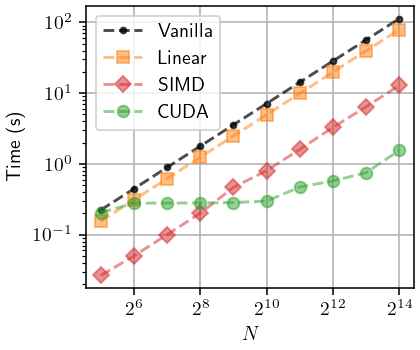
\includegraphics[width=.8\textwidth]{img/desktop/abs_performance-N.png}
        \caption{Absolute runtime with $P = 2^{10}$.}
    \end{subfigure}
    \begin{subfigure}{.49\textwidth}
        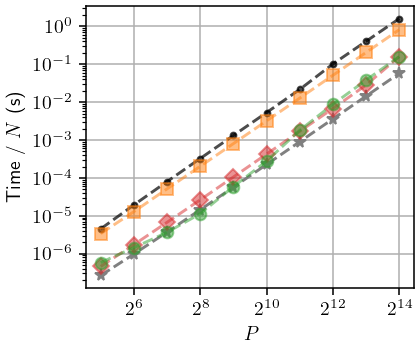
\includegraphics[width=.8\textwidth]{img/desktop/abs_performance-pP.png}
        \caption{Absolute runtime with $N = 2^{10}$.}
    \end{subfigure}\\
    \begin{subfigure}{.49\textwidth}
        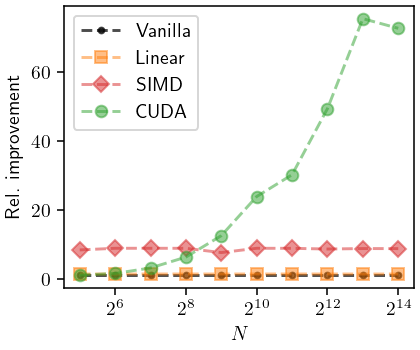
\includegraphics[width=.8\textwidth]{img/desktop/rel_performance-N.png}
        \caption{Relative improvement with $P = 2^{10}$.}
    \end{subfigure}
    \begin{subfigure}{.49\textwidth}
        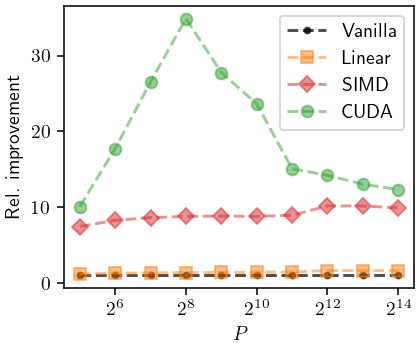
\includegraphics[width=.8\textwidth]{img/desktop/rel_performance-pP.png}
        \caption{Relative improvement with $N = 2^{10}$.}
    \end{subfigure}
    \caption{Comparison of four different implementations of the Fast Fr\'echet Distance algorithm on a laptop (CPU: AMD Ryzen Threadripper 3960X, GPU: NVIDIA GeForce RTX 3090 (24\,GB VRAM), CUDA Version: 12.2) using 32-bit floating point numbers. \textit{Vanilla} and \textit{Linear} refer to Alg.~\ref{alg:no_recursion} and \ref{alg:linear}, respectively. The SIMD implementation uses a batch size of $B = 16$ (twice the size of a 256-bit register in order to improve the instruction level parallelism) and relies on the AVX2 instruction set; the baseline implementation uses the same technique to calculate $\sum_{ij} d_{ij}$. The CUDA implementation uses a grid and block size of 128 and 64, respectively, that was measured to perform best for $N=2^{13}$ and $P=2^{10}$. All variants utilize only a single CPU core.}
    \label{fig:benchmark_desktop}
\end{figure}
